%intel-xeon-x5650 = 2.1 GFLOPS/core
%six cores

%m2090 = 665 GFLOPS
\documentclass[11pt, twocolumn]{article}
\usepackage[T1]{fontenc}
\usepackage{mathptmx}
\hyphenpenalty=5000
\usepackage{graphicx}
\usepackage[dvips,letterpaper,nohead,margin=.7in]{geometry} 
\usepackage[numbers]{natbib}
\usepackage{amsmath}
\selectfont

\setlength\parskip{0.1in}

\author{Gavin Gresham}
\title{Comparison of MPI, OpenMP and CUDA on the SUMMA algorithm on varying matrix dimensions and block sizes}

\begin{document}
\maketitle
%%%%%%%%%%%%%%%%%%%%%%%%%%%%%%%%%%%%%%%%%%%%%%%%%%%%%%%%%%%%
\section{Overview}
The goal of this paper is to compare matrix multiplication performance of three implementations. These consist of a base SUMMA algorithm, SUMMA+OpenMP, and SUMMA+CUDA. Additionally, the impact of matrix size and panel block size on these implementations will be analyzed. These results will be evaluated and used to answer questions about the nature of the implementations.

All tests will be performed on the Jinx cluster using four nodes. SUMMA and SUMMA+OpenMP will both use the same number of threads for comparison, while SUMMA+CUDA will use the 4 nodes and 8 GPUs. Performance will be judged using GFLOPS.


%%%%%%%%%%%%%%%%%%%%%%%%%%%%%%%%%%%%%%%%%%%%%%%%%%%%%%%%%%%%
\section{Implementation}
\subsection{MPI}
The base MPI implementation was done to implement the SUMMA algorithm\cite{SUMMA}. $N$ number of nodes are started and the $A$ and $B$ matrices are subdivided and allocated to these nodes evenly. A reference to a segment of the resultant $C$ matrix is also passed in to the summa function to be computed and recombined at the end of the program.

Within each node several variables are first calculated. The MPI rank of the node is retrieved and its relative $X$ and $Y$ coordinate in the processor grid is determined(Eqn \ref{nodeCoordsX}, \ref{nodeCoordsY}). From this information, the dimensions of the block this node is responsible for are calculated. Temporary buffers are allocated for the $A$ and $B$ buffer based on their row length, and the broadcast size. These buffers will be used with $MPI_Bcast$ later in the code.

\begin{eqnarray}
\label{nodeCoordsX}
Node_X = rank \% Grid_Y\\
\label{nodeCoordsY}
Node_Y = rank / Grid_Y
\end{eqnarray}

Next, new $MPI\_Comm$ communicators are set up in order to use MPI's more efficient broadcast method. The groups are assigned using the coordinates found using the node's rank found previously. With the communicator set up, the main loop is ready to begin.

The main loop moves through all the paired column and row nodes in sequence. Within this loop, there is another loop that waits until all of the data from the nodes have been broadcast and received. The number of iterations of this inner loops depends on the panel block size.

Before the algorithm transmits or receives any new data, the temporary buffers are first reset to 0. Next, the relevent columns are copied into $A$'s temporary buffer from $A$. Because $A$ is in column major format this is a simple $memcpy$. $B$ however, has to be stored in a reordered buffer in order to be broadcast correctly.

The $MPI\_Bcast$ method is now called for both $A$ on the $rowComm$ and $B$ on the $colComm$ (Fig \ref{fig:Comms}). The sending node is determined by the outer loop; All other nodes instead receive data to their temporary buffers. Once that is complete, the temporary data for $B$ has to be reordered once again to fit into column major order.

\begin{figure}[h]
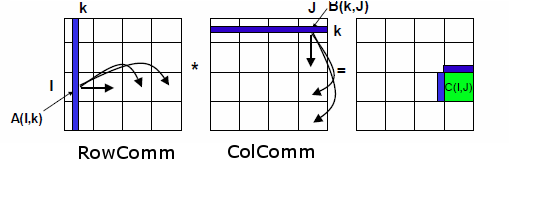
\includegraphics[scale=.5]{Images/Comms.png}
\caption{The data each node broadcasts using $rowComm$ and $colComm$. Original image from \cite{COMMS_FIG}}
\label{fig:Comms}
\end{figure}

Finally, local matrix multiply is performed on the temporary buffers and the results are added to $C$.

This process continues until all the data from this pair of nodes is sent ($Block_K / PanelBlockSize$ iterations). The algorithm then moves to the next pair of nodes and repeats the process.
%%%%%%%%%%%%%%%%%%%%%%%%%%%%%%%%%%%%%%%%%%%%%%%%%%%%%%%%%%%%
\subsection{OpenMP}
\subsubsection{Na�ve}
The initial implementation of OpenMP is very straight forward. The outer loop of the local matrix multiple was parallelized allowing each column to be computed independantly of the others. The $row$ and $col$ variables were made constant so the threads would not interfere with each other.

\subsubsection{Loop unrolling and blocking}
This is where the more significant optimizations occur. It includes the same additions from the na�ve implementation, but also other improvements to help with cache misses and pre-fetching.

First, I unrolled the loop so that it performs four steps each iteration. The idea is to reduce the loop overhead in the form of branch mispredictions. Additionally, creating new variables for these four steps should help alleviate any Write-After-Write (WAW) stalls that were occuring in the processor pipeline. The four counter variables are combined after each interloop and this final dot product is added to $C$.

%TODO: Blocking
%%%%%%%%%%%%%%%%%%%%%%%%%%%%%%%%%%%%%%%%%%%%%%%%%%%%%%%%%%%%
\subsection{CUDA}
\subsubsection{Host}
The CUDA implementation expands upon the SUMMA algorithm by replace the normal local matrix multiply with one that computes the results on the GPU, rather than the CPU.

Before any benchmark is run, the system is first queried for information on the GPUs. Primarily, how many GPUs are available, and what is the size of their shared memory. This takes a a non-trivial amount of time so should not be done within the first benchmark test, as it will skew the results.

Once the local multiplication method is called, the matrix is split into segments based on how many GPUs are available. Memory is then allocated on each device for matrices $A$, $B$, and $C$. The host copy of the matrices are transferred to this memory on the device.

Using the information on shared memory the maximum number of rows that can fit in a block's shared memory is computed. This allows for a better allocation of blocks for the CUDA kernel, and better scalability. The kernel is then launched with this number of blocks, one thread per matrix element, and enough shared memory to store local copies of the matrices.

%New section?
After the kernel is done executing, $C$ is copied from the device to host, and the matrix arrays on the device are freed.

\subsubsection{Device}
The shared memory is first divided into two arrays. One for $A$ and the other for $B$. Each thread then copies the matrix element it is responsible for from  global memory to the shared arrays for $A$ and $B$. These reads are made in a way that should allow for coalesced memory access as per \cite{CUDA_PGUIDE}, resulting in a minimal number of memory transactions. There is a $\_\_syncthread()$ call after this procedure to ensure the shared memory is in place before proceeding.

The thread then determines its row and column by using the built in CUDA $threadIdx$ and $blockIdx$ structures to find its place within the grid. Knowing its row and column, the thread can perform the innermost loop of the standard local multiplication loading each required element from the shared array. The final dotproduct is written to the corresponding element in $C$.

%%%%%%%%%%%%%%%%%%%%%%%%%%%%%%%%%%%%%%%%%%%%%%%%%%%%%%%%%%%%

\section{Evaluation}
The quality of the implementations is judged primarily on GFLOPS/s and future scalability. GFLOPS/s is acquired by comparing each implementations runtime against the GFLOPS of computing a matrix (Eqn \ref{eqn:GFLOPS}). This number is also compared agains the theoretical maximum GFLOPS of the given device.

\subsection{SUMMA}
The SUMMA algorithm performed adequately, though the results were not as impressive as I had hoped. With each core of the X5650 having performance around 2.1 GFLOPS \cite{XEON_FLOPS}, the max GFLOPS I could be achieving is 33.6 GFLOPS using 16 cores. Unfortunately, my implemenation falls well short of this.

The likely cause of performance loss is the overhead associated with MPI communication. MPI\_Bcast must block until data is received, making each thread only process as quickly as the slowest thread in the communicator. This also explains why increasing the panel block size increases performance. Fewer broadcasts results in less overhead and less time waiting. However, increasing the panel block size will increase the memory requirement of the threads, as the send and receive buffers will expand.

\begin{figure}[h]
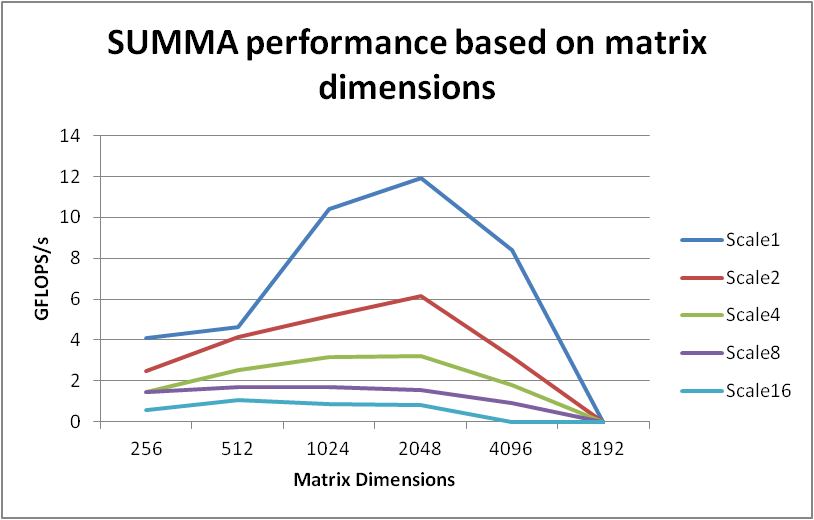
\includegraphics[scale=.3]{Images/SummaPerf.png}
\caption{The performance of the base SUMMA implementation based on matrix size and panel block size.}
\label{fig:SummaPerf}
\end{figure}

\subsection{OpenMP}
This implementation performed worse than I was expecting. Its performance closely matches that of the SUMMA implementation, often falling short.

This seems reasonable as the SUMMA implementation had a MPI process per core totalling 16 process on Jinx fourcore, while the OpenMP solution has one MPI process per Jinx node, and one OpenMP thread per core. Each implementation has 16 threads total, and have no real benefit over each other.

\subsection{CUDA}
The performance of the CUDA+SUMMA implementation was signficant after seeing the results of the previous two implementations. While very little benefit is gained from low panel block sizes (Tbl \ref{tbl:CUDA_PERF}), the more data that can be provided to the GPU, better the performance was. It not only continued to scale as the panel block size increased, but the GFLOPS increased at a rate greater than any other implementation.

\begin{figure}[htb]
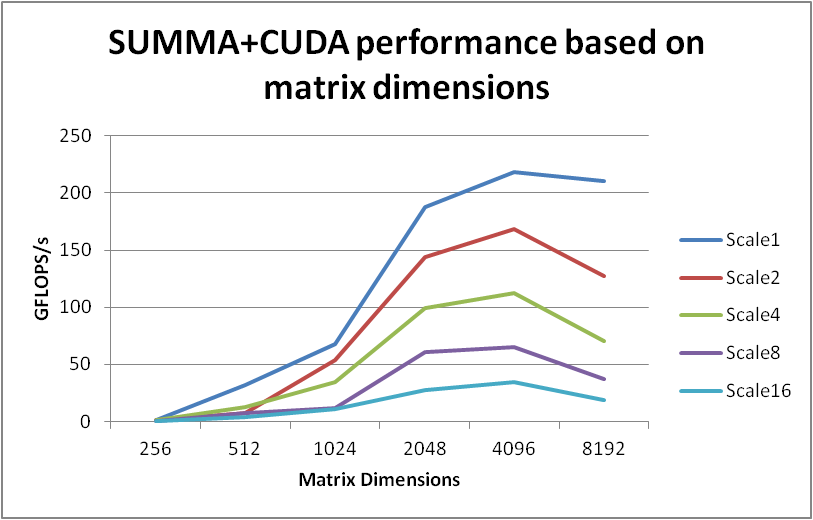
\includegraphics[scale=.3]{Images/CUDAPerf.png}
\caption{The performance of the CUDA+SUMMA implementation based on matrix size and panel block size$^1$.}
\label{fig:CUDAPerf}
\end{figure}

\begin{align}
\label{eqn:GFLOPS}
GFLOPS &= mn*2k\\
GFLOPS/s &= \frac{GFLOPS}{runtime}
\end{align}

\begin{table*}[tbh]
\centering
\begin{tabular}{|c|c|c|c|c|}
\hline
Matrix Dimensions & Panel Block Size\footnotemark[1] & Timer per Iteration (s) & GFLOPS & \% of theoretical max\\\noalign{\hrule height 1pt}
256 & 128 & 0.035 & 0.9441 & 0.071\\\hline
512 & 256 & 0.008 & 31.517 & 2.369\\\hline
1024 & 512 & 0.031 & 68.061 & 5.117\\\hline
2048 & 1024 & 0.091 & 187.197& 14.075\\\hline
4096 & 1024 & 0.628 & 218.558 & 16.432\\\hline
8192 & 512 & 5.218 & 210.706 & 15.842\\\hline
\end{tabular}
\caption{Shows the correlation between the Matrix size, the panel block size, and the performance of the CUDA implementation measured in GFLOPS/s}
\label{tbl:CUDA_PERF}
\end{table*}

\begin{table*}[tbh]
\centering
\begin{tabular}{|c|c|c|c|}
\hline
Matrix Dimensions & GFLOPS & Time per Iteration (s) & \% of theoretical max\\\noalign{\hrule height 1pt}
256 & 0.013 & 2.4275 & 0.182\\\hline
512 & 0.005 & 47.823 & 3.595\\\hline
1024 & 0.0138 & 155.8401 & 11.717\\\hline
2048 & 0.040 & 428.9813 & 32.254\\\hline
4096 & 0.162 & 846.361 & 63.636\\\hline
\end{tabular}
\caption{The performance of my CUDA implementation on matrix multiplication without SUMMA}
\label{tbl:CUDA_MM_PERF}
\end{table*}
%%%%%%%%%%%%%%%%%%%%%%%%%%%%%%%%%%%%%%%%%%%%%%%%%%%%%%%%%%%%
\section{Conclusion}
\subsection{Best Performance}
\begin{figure}[htb]
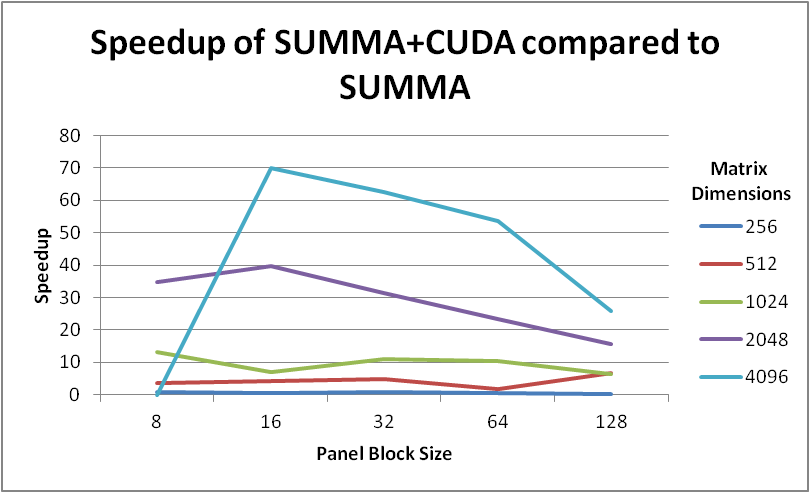
\includegraphics[scale=.3]{Images/CUDASpeedup.png}
\caption{The performance gain of CUDA+SUMMA over the base SUMMA implementation.}
\label{fig:CUDA_SPEEDUP}
\end{figure}

The implementation with the best performance in terms of time and GFLOPS/s is clearly SUMMA combined with CUDA. As seen in fig \ref{fig:CUDA_SPEEDUP}, in almost all cases the addition of CUDA greatly increases the GFLOPS while reducing the time needed to compute the matrix multiplication. 

While the matrix sizes grow the performance does as well. This is due to an underutilization of the GPU. Using $mn*2k$ we can determine the GFLOP required to multiply given matrices. A matrix size of 4096 equates to ~137 GFLOP; well below the 665 GFLOPS performance of a single NVIDIA m2090 \cite{TECH_SPEC}. This is with a single GPU. 

Given that each Jinx node contains two NVIDIA m2090's \cite{JINX_INFO}, and I used 4 nodes in my implementation, the maximum theoretical GFLOPS is 5320. Using eqn \ref{eqn:GFLOPS}, a matrix would need dmensions of nearly 14,000 to reach that threshold.

\subsection{Most Scalable}
I believe that once again the combination of SUMMA and CUDA comes out ahead of the other implementations. While the other algorithms failed to complete larger matrices in the allotted time, the GPUs were able to compute the 8192 dimension matrix in under 60 seconds even in the worst case.

The bottleneck did not come in the way of processing power, but memory. Assuming a double precision float takes 8 bytes, $A$, $B$, and $C$ will take 1.6 Gigabytes of memory \ref{eqn:MatrixSizes}. Despite GPU nodes on Jinx having 24GB of memory \cite{JINX_INFO}, my executables could not allocated over 2GB. I'm unsure why this is as the executable is 64-bit and no stack trace is returned.

The number of GPUs that a node can use is not bound so this will scale as more GPUs are added to a system. Additionally, the shared memory of each CUDA block is queried on startup, ideally allowing for an optimal allocation of blocks for any GPU. As long as no hard limits are hit in terms of memory, I don't see a reason this implementation could not scale to much larger matrices.

\begin{equation}\label{eqn:MatrixSizes}
8\; bytes * 8192^2 * 3= 1,610,612,736 bytes
\end{equation}

\subsection{Line Estimates}
The lines of the SUMMA implementation are about 140 lines. The MPI changes are an additional 30. The CUDA implementation is about 140 lines of code in addition to the SUMMA changes.
\subsection{Most Complex Problem of the Implementation}
I believe the most complex part of the implementation was the actual SUMMA algorithm. It was difficult for me to visualize the interactions between separate nodes coordinating their broadcasts and keeping the data in order. 

A close second was the actual CUDA kernel. The idea of SIMD was hard to grasp at first, trying to understand thousands of threads working in parallel. This in addition to the optimizations that are required to make CUDA worthwhile was complex.
%%%%%%%%%%%%%%%%%%%%%%%%%%%%%%%%%%%%%%%%%%%%%%%%%%%%%%%%%%%%

\footnotetext[1]{Due to memory constraints the panel block size of matrices sized 8196 had to be reduced. This is a likely cause of performance decrease for these matrices.}

\bibliography{Summa}
\bibliographystyle{plainnat}
\end{document}
